163. \begin{figure}[ht!]
\center{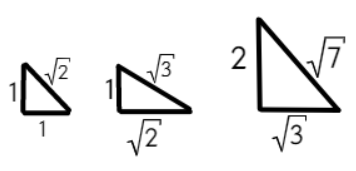
\includegraphics[scale=0.35]{g8-163.png}}
\end{figure}\\
Будем использовать стандартные построения, позволяющее восстанавливать перпендикуляр в точке и откладывать отрезок, равный данному. Сначала построим перпендикулярные отрезки длины 1, по теореме Пифагора получим третий отрезок длины $\sqrt{2}.$ Затем аналогично построим отрезки длины $\sqrt{3}$ и $\sqrt{7}.$
ewpage
oindent
